\documentclass[12pt]{report}
\usepackage[utf8]{inputenc}
\usepackage[russian]{babel}
%\usepackage[14pt]{extsizes}
\usepackage{listings}
\usepackage{graphicx}
\usepackage{amsmath,amsfonts,amssymb,amsthm,mathtools} 
\usepackage{pgfplots}
\usepackage{filecontents}
\usepackage{float}
\usepackage{indentfirst}
\usepackage{eucal}
\usepackage{enumitem}
\frenchspacing

\usepackage{indentfirst} % Красная строка


\usetikzlibrary{datavisualization}
\usetikzlibrary{datavisualization.formats.functions}

\usepackage{amsmath}




% Для листинга кода:
\lstset{ %
language=haskell,                 % выбор языка для подсветки (здесь это С)
basicstyle=\small\sffamily, % размер и начертание шрифта для подсветки кода
numbers=left,               % где поставить нумерацию строк (слева\справа)
numberstyle=\tiny,           % размер шрифта для номеров строк
stepnumber=1,                   % размер шага между двумя номерами строк
numbersep=5pt,                % как далеко отстоят номера строк от подсвечиваемого кода
showspaces=false,            % показывать или нет пробелы специальными отступами
showstringspaces=false,      % показывать или нет пробелы в строках
showtabs=false,             % показывать или нет табуляцию в строках
frame=single,              % рисовать рамку вокруг кода
tabsize=2,                 % размер табуляции по умолчанию равен 2 пробелам
captionpos=t,              % позиция заголовка вверху [t] или внизу [b] 
breaklines=true,           % автоматически переносить строки (да\нет)
breakatwhitespace=false, % переносить строки только если есть пробел
escapeinside={\#*}{*)}   % если нужно добавить комментарии в коде
}

\usepackage[left=2cm,right=2cm, top=2cm,bottom=2cm,bindingoffset=0cm]{geometry}
% Для измененных титулов глав:
\usepackage{titlesec, blindtext, color} % подключаем нужные пакеты
\definecolor{gray75}{gray}{0.75} % определяем цвет
\newcommand{\hsp}{\hspace{20pt}} % длина линии в 20pt
% titleformat определяет стиль
\titleformat{\chapter}[hang]{\Huge\bfseries}{\thechapter\hsp\textcolor{gray75}{|}\hsp}{0pt}{\Huge\bfseries}


% plot
\usepackage{pgfplots}
\usepackage{filecontents}
\usetikzlibrary{datavisualization}
\usetikzlibrary{datavisualization.formats.functions}

\begin{document}
%\def\chaptername{} % убирает "Глава"
\thispagestyle{empty}
\begin{titlepage}
	\noindent \begin{minipage}{0.15\textwidth}
	
\includegraphics[width=\linewidth]{img/b_logo}
	\end{minipage}
	\noindent\begin{minipage}{0.9\textwidth}\centering
		\textbf{Министерство науки и высшего образования Российской Федерации}\\
		\textbf{Федеральное государственное бюджетное образовательное учреждение высшего образования}\\
		\textbf{~~~«Московский государственный технический университет имени Н.Э.~Баумана}\\
		\textbf{(национальный исследовательский университет)»}\\
		\textbf{(МГТУ им. Н.Э.~Баумана)}
	\end{minipage}
	
	\noindent\rule{18cm}{3pt}
	\newline\newline
	\noindent ФАКУЛЬТЕТ $\underline{\text{«Информатика и системы управления»}}$ \newline\newline
	\noindent КАФЕДРА $\underline{\text{«Программное обеспечение ЭВМ и информационные технологии»}}$\newline\newline\newline\newline\newline
	
	
	\begin{center}
		\noindent\begin{minipage}{1.3\textwidth}\centering
			\Large\textbf{  Отчет по лабораторной работе №4}\newline
			\textbf{по дисциплине "Операционные системы"}\newline\newline
		\end{minipage}
	\end{center}
	
	\noindent\textbf{Тема} $\underline{\text{Процессы. Системные вызовы fork() и exec()}}$\newline\newline
	\noindent\textbf{Студент} $\underline{\text{Криков А.В.~~~~~~~~~~~~~~~~~~~~~~~~~~~~~~~~~~~~~~}}$\newline\newline
	\noindent\textbf{Группа} $\underline{\text{ИУ7-53Б~~~~~~~~~~~~~~~~~~~~~~~~~~~~~~~~~~~~~~~~~~~~~~}}$\newline\newline
	\noindent\textbf{Оценка (баллы)} $\underline{\text{~~~~~~~~~~~~~~~~~~~~~~~~~~~~~~~~~~~~~~~~~~~~~}}$\newline\newline
	\noindent\textbf{Преподаватели} $\underline{\text{Рязанова Н.Ю.~~~~~~~~~~~~~~~~~~~~~~~~~~}}$\newline\newline\newline
	
	\begin{center}
		\vfill
		Москва~---~\the\year
		~г.
	\end{center}
\end{titlepage}

\newpage

\section*{Задание №1}

Процессы-сироты. В программе создаются не менее двух потомков. В потомках вызывается sleep(). Чтобы предок гарантированно завершился раньше своих помков. Продемонстрировать с помощью соответствующего вывода информацию об идентификаторах процессов и их группе.

\begin{lstlisting}[label=some-code,caption=Процессы-сироты,language=C]
#include <stdio.h>
#include <unistd.h>



int main()
{
	printf("PARENT: PID = %d, GRP = %d\n", getpid(), getpgrp());
	int childpid1, childpid2;

	if ((childpid1 = fork()) == 1)
	{
		perror("Not forked child 1!\n");
		return 1;
	} 
	else if (childpid1 == 0) 
	{
		printf("lock: PID = %d, GRP = %d PPID = %d\n", getpid(), getpgrp(), getppid());
		sleep(5);
		printf("unlock: PID = %d, GRP = %d PPID = %d\n", getpid(), getpgrp(), getppid());
		return 0;
	}

	if ((childpid2 = fork()) == 1)
	{
		perror("Not forked child 2!\n");
		return 1;
	} 
	else if (childpid2 == 0) 
	{
		printf("lock: PID = %d, GRP = %d PPID = %d\n", getpid(), getpgrp(), getppid());
		sleep(10);
		printf("unlock: PID = %d, GRP = %d PPID = %d\n", getpid(), getpgrp(), getppid());
		return 0;
	}

	printf("Parent: id: %d pgrp: %d child1: %d child2: %d\n", getpid(), getpgrp(), childpid1, childpid2);
	printf("Parent died!\n\n");
	return 0;
}
\end{lstlisting}

\begin{figure}[H]

	\centering

	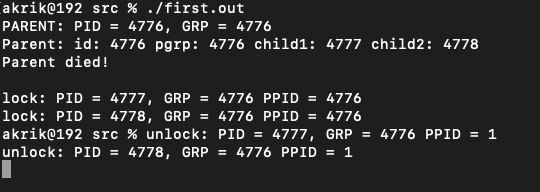
\includegraphics[width=\linewidth]{img/first.png}
	\caption{Демонстрация работы программы (задание №1).}

	\label{fig:task01}

\end{figure}

\section*{Задание №2}

Предок ждет завершения своих потомком, используя системный вызов
wait(). Вывод соответствующих сообщений на экран.

\begin{lstlisting}[label=some-code,caption=Вызов функции wait(),language=C]
#include <stdio.h>
#include <unistd.h>
#include <sys/wait.h>
#include <stdlib.h>

void check_status(int status);

int main()
{
	printf("PARENT: PID = %d, GRP = %d\n\n", getpid(), getpgrp());
	int childpid1, childpid2;

	if ((childpid1 = fork()) == 1)
	{
		perror("Not forked child 1!\n");
		return 1;
	}
	else if (childpid1 == 0) 
	{
		printf("CHILD_1 : PID = %d, GRP = %d PPID = %d\n", getpid(), getpgrp(), getppid());
		sleep(5);
		return 0;
	}

	if ((childpid2 = fork()) == 1)
	{
		perror("Not forked child 2!\n");
		return 1;
	} 
	else if (childpid2 == 0) 
	{
		printf("CHILD_2 : PID = %d, GRP = %d PPID = %d\n", getpid(), getpgrp(), getppid());
		sleep(7);
		return 0;
	}

	int status;
	pid_t childpid;

	childpid = wait(&status);
	printf("STATUS = %d,  CHILD_PID = %d\n", status, childpid);
	check_status(status);

	childpid = wait(&status);
	printf("STATUS = %d,  CHILD_PID = %d\n", status, childpid);
	check_status(status);

	printf("Parent: id: %d pgrp: %d\n", getpid(), getpgrp());
	printf("Parent died!\n\n");

	return 0;
}
	
	
void check_status(int status)
{
	if (WIFEXITED(status))
	{
		printf("The child process is completed normally.\n");
		printf("Child process termination code %d.\n\n", WEXITSTATUS(status));
		return;
	}

	if (WIFSIGNALED(status))
	{
		printf("The child process terminates with an un-intercepted signal.\n");
		printf("Signal number %d.\n", WTERMSIG(status));
		return;
	}

	if (WIFSTOPPED(status))
	{
		printf("The child process has stopped.\n");
		printf("Signal number %d.", WSTOPSIG(status));
	}
}
\end{lstlisting}

\begin{figure}[H]

	\centering

	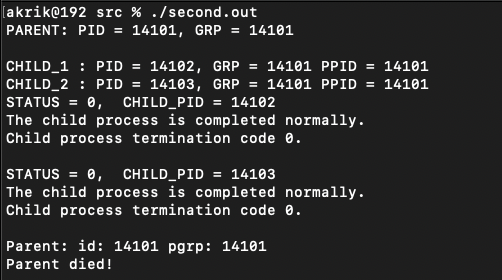
\includegraphics[width=\linewidth]{img/second.png}
	\caption{Демонстрация работы программы (задание №2).}

	\label{fig:task02}

\end{figure}

\section*{Задание №3}

Потомки переходят на выполнение других программ. Предок ждет завершения своих потомков. Вывод соответствующих сообщений на экран.\newline

execl первого потомка использует программу сортировки массива слиянием.


execl второго потомка использует программу для поиска значения функции с помощью интерполяции полиномом Ньютона.\newline

Параметры передаваемые в execl для первого потомка:


1 - название исполняемого файла 


2 - размер входного неотсортированного массива


3..7 - входной неотсортированный массив\newline


Параметры передаваемые в execl для второго потомка:

1 - название исполняемого файла 

2 - файл, содержащий в себе промежуточные значения произвольной функции 

3 - значение аргумента, для которого нужно найти значение функции

4 - степень интерполяционного полинома






\begin{lstlisting}[label=some-code,caption=Вызов функции execl(),language=C]
#include <stdio.h>
#include <unistd.h>
#include <sys/wait.h>
#include <stdlib.h>

void check_status(int status);

int main()
{
	printf("PARENT: PID = %d, GRP = %d\n\n", getpid(), getpgrp());
	int childpid1, childpid2;
	int status;
	pid_t childpid;


	if ((childpid1 = fork()) == 1)
	{
		perror("Not forked child 1!\n");
		return 1;
	} 
	else if (childpid1 == 0) 
	{
		printf("CHILD_1 : PID = %d, GRP = %d PPID = %d\n\n", getpid(), getpgrp(), getppid());

        if (execl("merge_sort.out", "5", "19", "12", "14", "11", "42", NULL) == -1)
		{
			perror("CHILD_1 cant exec");
			return 1;
		}

		return 0;
	}

	if ((childpid2 = fork()) == 1)
	{
		perror("Not forked child 2!\n");
		return 1;
	} 
	else if (childpid2 == 0) 
	{
		printf("CHILD_2 : PID = %d, GRP = %d PPID = %d\n\n", getpid(), getpgrp(), getppid());

        if (execl("newton_interpolation.out", "func.txt", "0.4", "4", NULL) == -1)
		{
			perror("CHILD_2 cant exec");
			return 1;
		}

		return 0;
	}

	childpid = wait(&status);
	check_status(status);

	childpid = wait(&status);
	check_status(status);

	printf("Parent: id: %d pgrp: %d child1: %d child2: %d\n", getpid(), getpgrp(), childpid1, childpid2);
	printf("Parent died!\n\n");

	return 0;
}


void check_status(int status)
{
	if (WIFEXITED(status))
	{
		printf("The child process is completed normally.\n");
		printf("Child process termination code %d.\n\n", WEXITSTATUS(status));
		return;
	}

	if (WIFSIGNALED(status))
	{
		printf("The child process terminates with an un-intercepted signal.\n");
		printf("Signal number %d.\n", WTERMSIG(status));
		return;
	}

	if (WIFSTOPPED(status))
	{
		printf("The child process has stopped.\n");
		printf("Signal number %d.", WSTOPSIG(status));
	}
}
\end{lstlisting}

\begin{figure}[H]

	\centering

	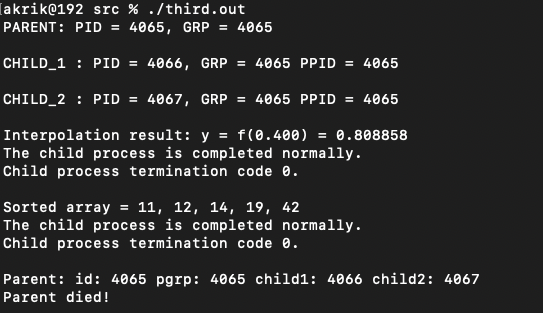
\includegraphics[width=\linewidth]{img/third.png}
	\caption{Демонстрация работы программы (задание №3).}

	\label{fig:task03}

\end{figure}

\section*{Задание №4}

Предок и потомки обмениваются сообщениями через неименованный
программный канал. Предок ждет завершения своих потомков. Вывод соответствующих сообщений на экран.

\begin{lstlisting}[label=some-code,caption=Использование pipe,language=C]
#include <stdio.h>
#include <stdlib.h>
#include <sys/wait.h>
#include <unistd.h>
#include <string.h>


void check_status(int status);

int main()
{
	int childpid1, childpid2;
	int fd[2];
	char first_text[57] = "Tyger Tyger, burning bright, In the forests of the night";
  char second_text[44] = "The forest paths are muddy, after the rain.";

	if (pipe(fd) == -1) 
	{
		perror("Cant pipe.\n");
		return 1;
	}

	if ((childpid1 = fork()) == -1)
	{
		perror("Not forked.\n");
		return 1;
	}
	else if (!childpid1) 
	{
		close(fd[0]);
		write(fd[1], first_text, strlen(first_text) + 1);

        printf("First child message send to parent, message: %s\n", first_text);      

		return 0;

	}

	if ((childpid2 = fork()) == -1)
	{
		perror("Not forked.\n");
		return 1;
	}
	else if (!childpid2)
	{
		close(fd[0]);
		write(fd[1], second_text, strlen(second_text) + 1);

        printf("Second child message send to parent, message: %s\n\n", second_text);

		return 0;
	}

	if (childpid1 && childpid2)
	{
		char text1[57], text2[44];
		pid_t childpid;
		int status;

		close(fd[1]);

		read(fd[0], text1, strlen(first_text) + 1);
		read(fd[0], text2, strlen(second_text) + 1);

		printf("Text first: %s\n", text1);
		printf("Text second: %s\n\n", text2);

		childpid = wait(&status);
		check_status(status);

		childpid = wait(&status);
		check_status(status);

		printf("Parent: id: %d pgrp: %d child1: %d child2: %d\n", getpid(), getpgrp(), childpid1, childpid2);
    	printf("Parent died!\n\n");
	}

	return 0;
}

void check_status(int status)
{
	if (WIFEXITED(status))
	{
		printf("The child process is completed normally.\n");
		printf("Child process termination code %d.\n\n", WEXITSTATUS(status));
		return;
	}

	if (WIFSIGNALED(status))
	{
		printf("The child process terminates with an un-intercepted signal.\n");
		printf("Signal number %d.\n", WTERMSIG(status));
		return;
	}

	if (WIFSTOPPED(status))
	{
		printf("The child process has stopped.\n");
		printf("Signal number %d.", WSTOPSIG(status));
	}
}
\end{lstlisting}

\begin{figure}[H]

	\centering

	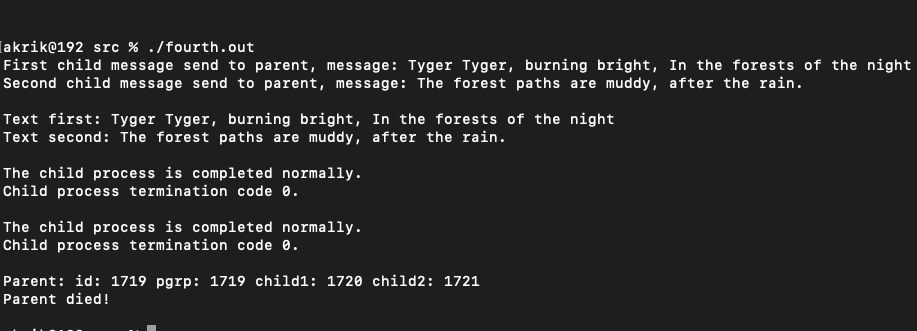
\includegraphics[width=\linewidth]{img/fourth.png}
	\caption{Демонстрация работы программы (задание №4).}

	\label{fig:task04}

\end{figure}

\section*{Задание №5}

Предок и потомки обмениваются сообщениями через неименованный программный канал. С помощью сигнала меняется ход выполнения программы. Предок ждет завершения своих потомков. Вывод соответствующих сообщений на экран.

\begin{lstlisting}[label=some-code,caption=Использование сигналов,language=C]
	#include <stdio.h>
	#include <stdlib.h>
	#include <sys/wait.h>
	#include <unistd.h>
	#include <signal.h>
	#include <stdbool.h>
	#include <string.h>
	
	
	_Bool flag = false;
	
	void check_status(int status);
	
	
	void catch_sig(int sig_numb)
	{
		flag = true;
		printf("catch_sig: %d\n", sig_numb);
	}
	
	
	int main()
	{
		signal(SIGINT, catch_sig);
	
		int childpid_1, childpid_2;
		int fd[2];
		char text1[57] = "\0", text2[44] = "\0";
		char first_text[57] = "Tyger Tyger, burning bright, In the forests of the night";
		char second_text[44] = "The forest paths are muddy, after the rain.";
		pid_t childpid;
		int status;
	
		printf("Parent: press CTRL+C if you want to see messages from childs\n\n");
		sleep(5);
	
		if (pipe(fd) == -1)
		{
			perror("Cant pipe.\n");
			return 1;
		}
	
		if ((childpid_1 = fork()) == -1)
		{
			perror("Not forked.\n");
			return 1;
		}
		else if (!childpid_1)
		{
			if (flag) {
				close(fd[0]);
				write(fd[1], first_text, strlen(first_text) + 1);
	
				printf("First child message send to parent, message: %s\n", first_text);
			}
	
			return 0;
		}
	
		if ((childpid_2 = fork()) == -1)
		{
			perror("Cant fork.\n");
			return 1;
		}
		else if (!childpid_2) 
		{
			if (flag) {
				close(fd[0]);
				write(fd[1], second_text, strlen(second_text) + 1);
	
				printf("Second child message send to parent, message: %s\n", second_text);
			}
	
			return 0;
		}
	
		if (childpid_1 && childpid_2)
		{
			close(fd[1]);
	
			read(fd[0], text1, strlen(first_text) + 1);
			read(fd[0], text2, strlen(second_text) + 1);
	
			printf("\nText: %s\n", text1);
			printf("Text: %s\n\n", text2);
		}
	 
		childpid = wait(&status);
		check_status(status);
	
		childpid = wait(&status);
		check_status(status);
	
		printf("Parent: id: %d pgrp: %d child1: %d child2: %d\n", getpid(), getpgrp(), childpid_1, childpid_2);
		printf("Parent died!\n\n");
	
		return 0;
	}
	
	
	
	void check_status(int status)
	{
		if (WIFEXITED(status))
		{
			printf("The child process is completed normally.\n");
			printf("Child process termination code %d.\n\n", WEXITSTATUS(status));
			return;
		}
	
		if (WIFSIGNALED(status))
		{
			printf("The child process terminates with an un-intercepted signal.\n");
			printf("Signal number %d.\n", WTERMSIG(status));
			return;
		}
	
		if (WIFSTOPPED(status))
		{
			printf("The child process has stopped.\n");
			printf("Signal number %d.", WSTOPSIG(status));
		}
	}
\end{lstlisting}




\begin{figure}[H]

	\centering

	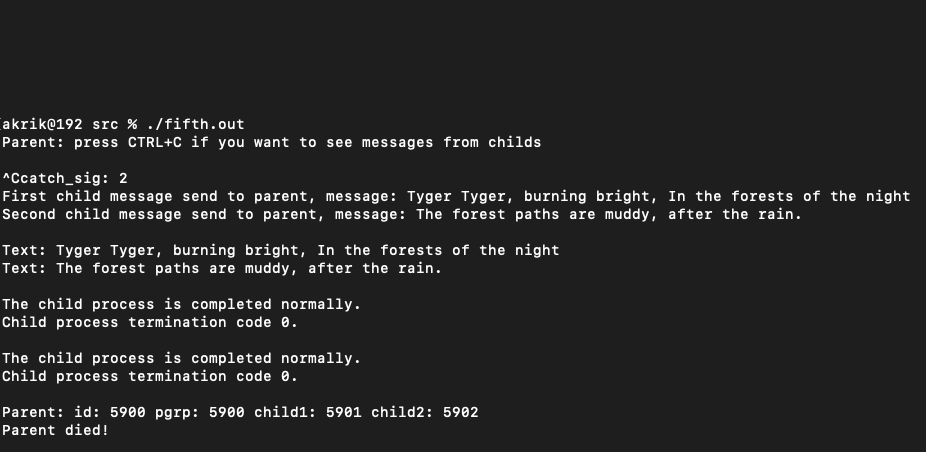
\includegraphics[width=\linewidth]{img/fifth.png}
	\caption{Демонстрация работы программы, сигнал = SIGINT (задание №5).}

	\label{fig:task05_01}

\end{figure}

\begin{figure}[H]

	\centering

	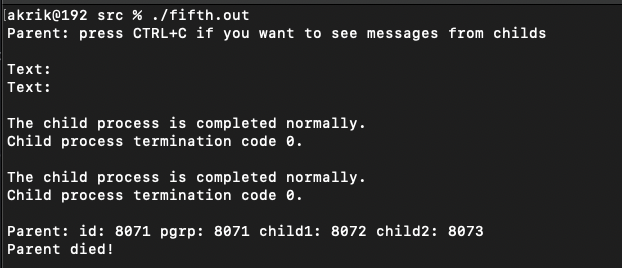
\includegraphics[width=\linewidth]{img/fifth2.png}
	\caption{Демонстрация работы программы, сигнал отсутствует (задание №5).}

	\label{fig:task05_02}

\end{figure}


\bibliographystyle{utf8gost705u}  % стилевой файл для оформления по ГОСТу

\bibliography{51-biblio}          % имя библиографической базы (bib-файла)

 

\section*{Дополнительное задание}

\begin{figure}[H]

	\centering

	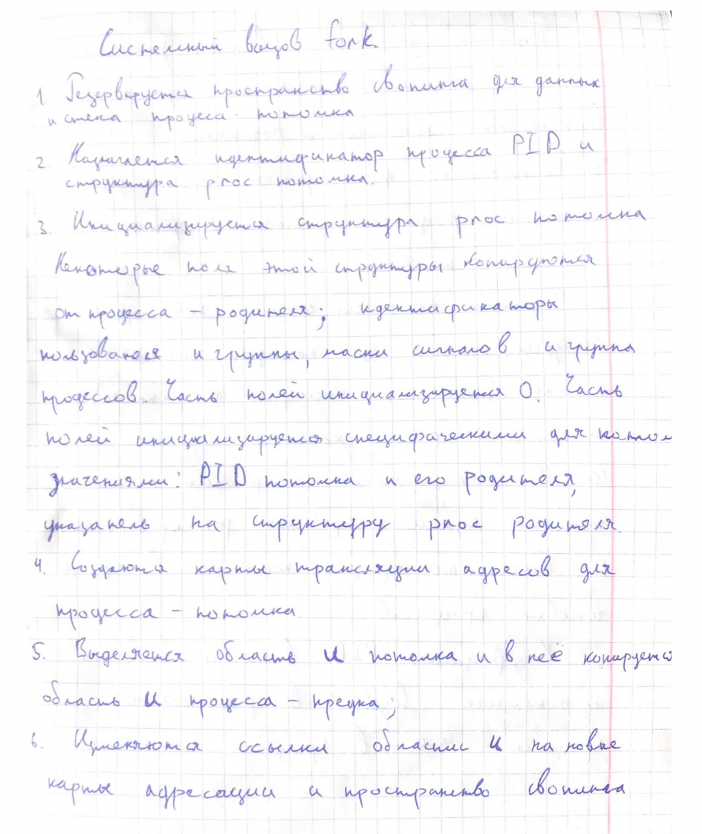
\includegraphics[width=\linewidth]{img/fork_1.png}
	\caption{Очередность действий при вызове fork (1)}

\end{figure}


\begin{figure}[H]

	\centering

	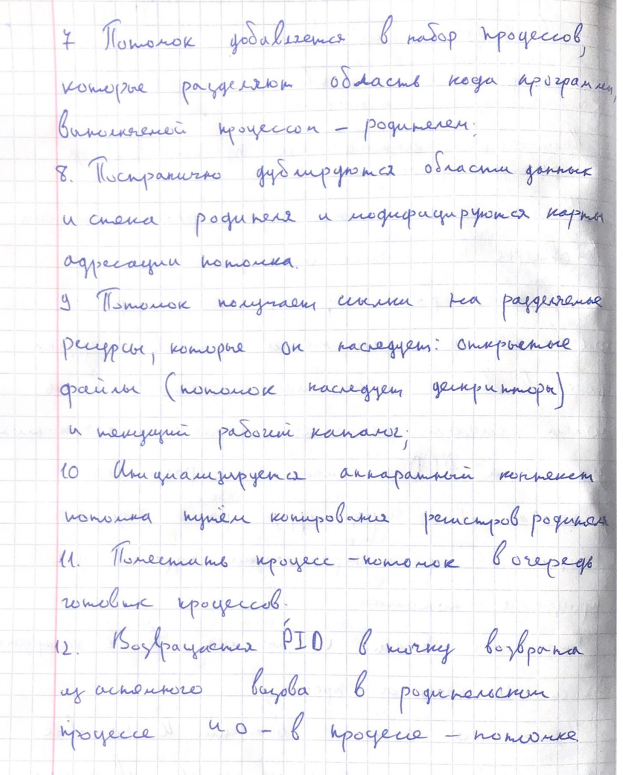
\includegraphics[width=\linewidth]{img/fork_2.png}
	\caption{Очередность действий при вызове fork (2)}

\end{figure}

\begin{figure}[H]

	\centering

	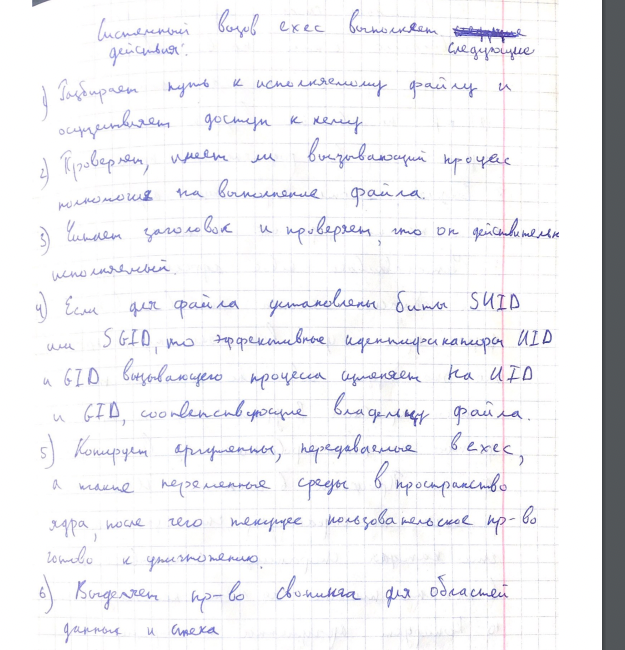
\includegraphics[width=\linewidth]{img/exec_1.png}
	\caption{Очередность действий при вызове exec (1)}

\end{figure}

\begin{figure}[H]

	\centering

	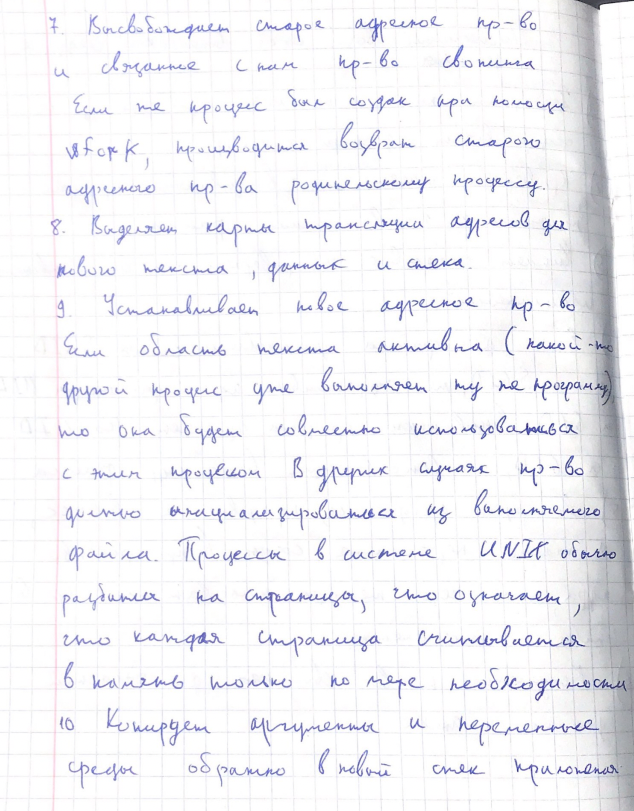
\includegraphics[width=\linewidth]{img/exec_2.png}
	\caption{Очередность действий при вызове exec (2)}

\end{figure}


\begin{figure}[H]

	\centering

	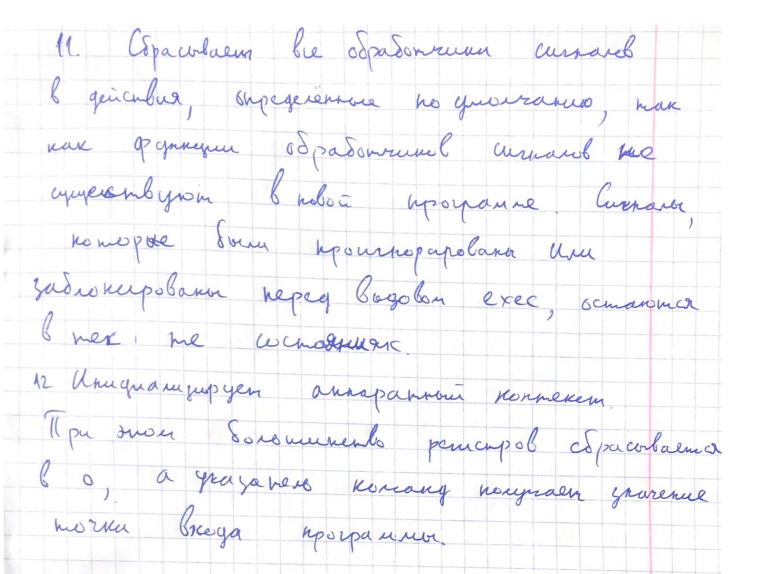
\includegraphics[width=\linewidth]{img/exec_3.png}
	\caption{Очередность действий при вызове exec (3)}

\end{figure}

\end{document}
